\section{Software Architektur}

\subsection{Services \& Komponenten}

Die Anwendung umfasst vier Microservices sowie ein Gateway.
In den folgenden Unterkapiteln werden Microservice und Gateway vorgestellt.

\subsubsection{Gateway}

Die Aufgabe des Gateways ist es eingehende Anfragen basierend auf Routing-Regeln weiterzuleiten.
Darüber hinaus befindet sich im Gateway auch die zentrale Swagger-UI-Dokumentationsplattform, auf welcher Endbenutzerinnen und Endbenutzer die REST-Schnittstellen der Microservices einsehen können.

\subsubsection{Entity-Service}

Die Aufgabe des Entity-Services ist es Metadaten sowie statische Daten von Entitäten zu verwalten.
Akteure registrieren sich bei diesem Service, um Teil der Simulation zu werden.
Über REST-Schnittellen können diese Daten abgefragt werden.

\subsubsection{Tracking-Service}

Die Aufgabe des Tracking-Services ist die Verwaltung von dynamischen Daten, welche von Entitäten generiert werden.
Während einer Simulation werden diese Daten an den Tracking-Service gesendet und von diesem im Anschluss persistiert.
Über REST-Schnittellen können diese Daten abgefragt werden.

\subsubsection{Simulator-Service}

Die Zentrale Aufgabe des Simulator-Services ist das Starten und Stoppen von Simulationen.
Sobald eine Simulation gestartet wurde, simuliert dieser Service Ampeln und Fahrzeuge.
Es registriert diese Akteure und spielt das Verhalten, welches im Algorithmus spezifiziert wurde, ab.

\subsubsection{Flowcontrol-Service}

Der Flowcontrol-Service berechnet optimalen Geschwindigkeit für Fahrzeuge basierend auf dem Zustand von Ampeln, sodass eine \textit{grüne Welle} erreicht wird. 

\subsection{Schnittstellen \& Kommunikation der Services}

\begin{figure}[h]
	\centering
	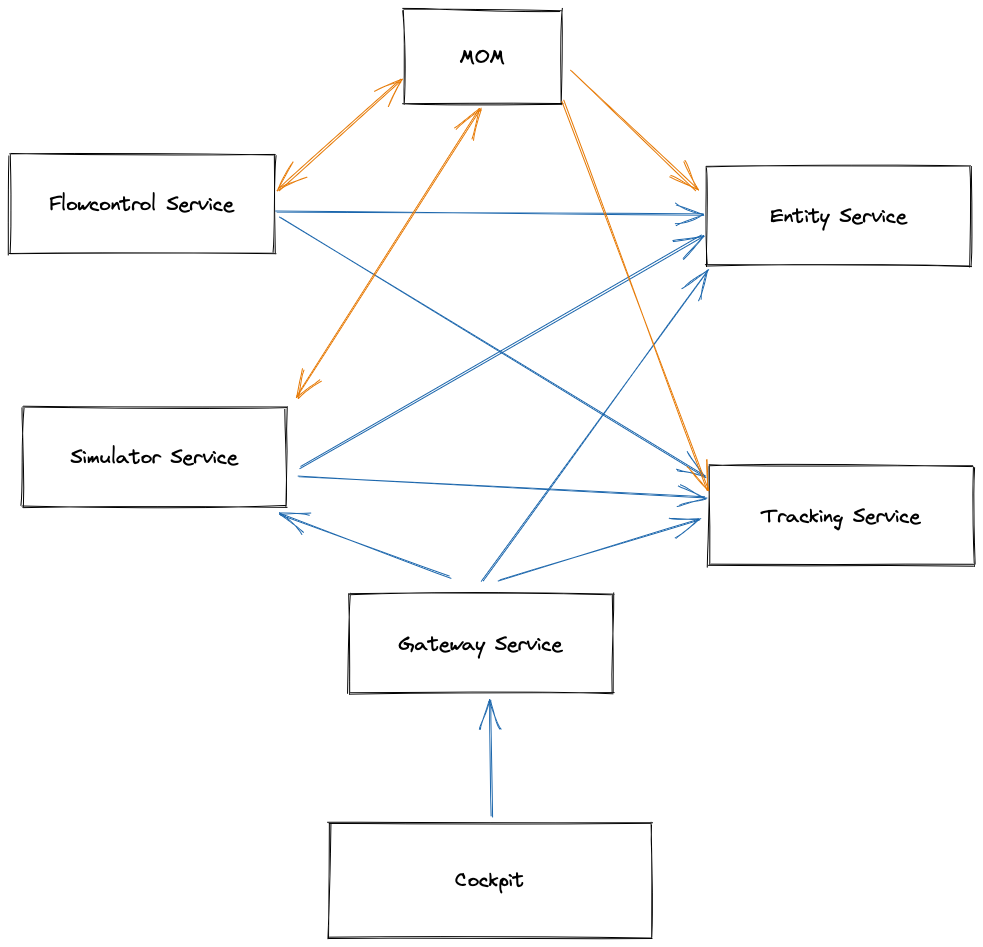
\includegraphics[width=1\textwidth]{./figures/whole_system_communication.png}
	\caption{Übersicht aller Schnittstellen und Kommunikationswege}
	\label{fig:wholesystem_view}
\end{figure}

Wie man der Abbildung \ref{fig:wholesystem_view} entnehmen kann, verfügt das System über zwei Arten von Schnittstellen.
Zuerst gibt es konventionelle synchrone REST-Schnittstellen (in Abbildung \ref{fig:wholesystem_view} mittels blauen Pfeilen dargestellt).
Darüber hinaus existieren asynchrone Schnittstellen (in Abbildung \ref{fig:wholesystem_view} mittels orangen Pfeilen dargestellt), welche mit einer Message Oriented Middleware (in diesem Falle RabbitMQ) realisiert wurden.
Grundsätzlich verwenden wir asynchrone Kommunikation, damit häufig stattfindender Datenaustausch nicht die Services blockiert.
Synchrone Kommunikation wird bei Operationen eingesetzt, welche nicht zeitkritisch sind oder synchron stattfinden müssen.

\subsubsection{REST}

\begin{figure}[h]
	\centering
	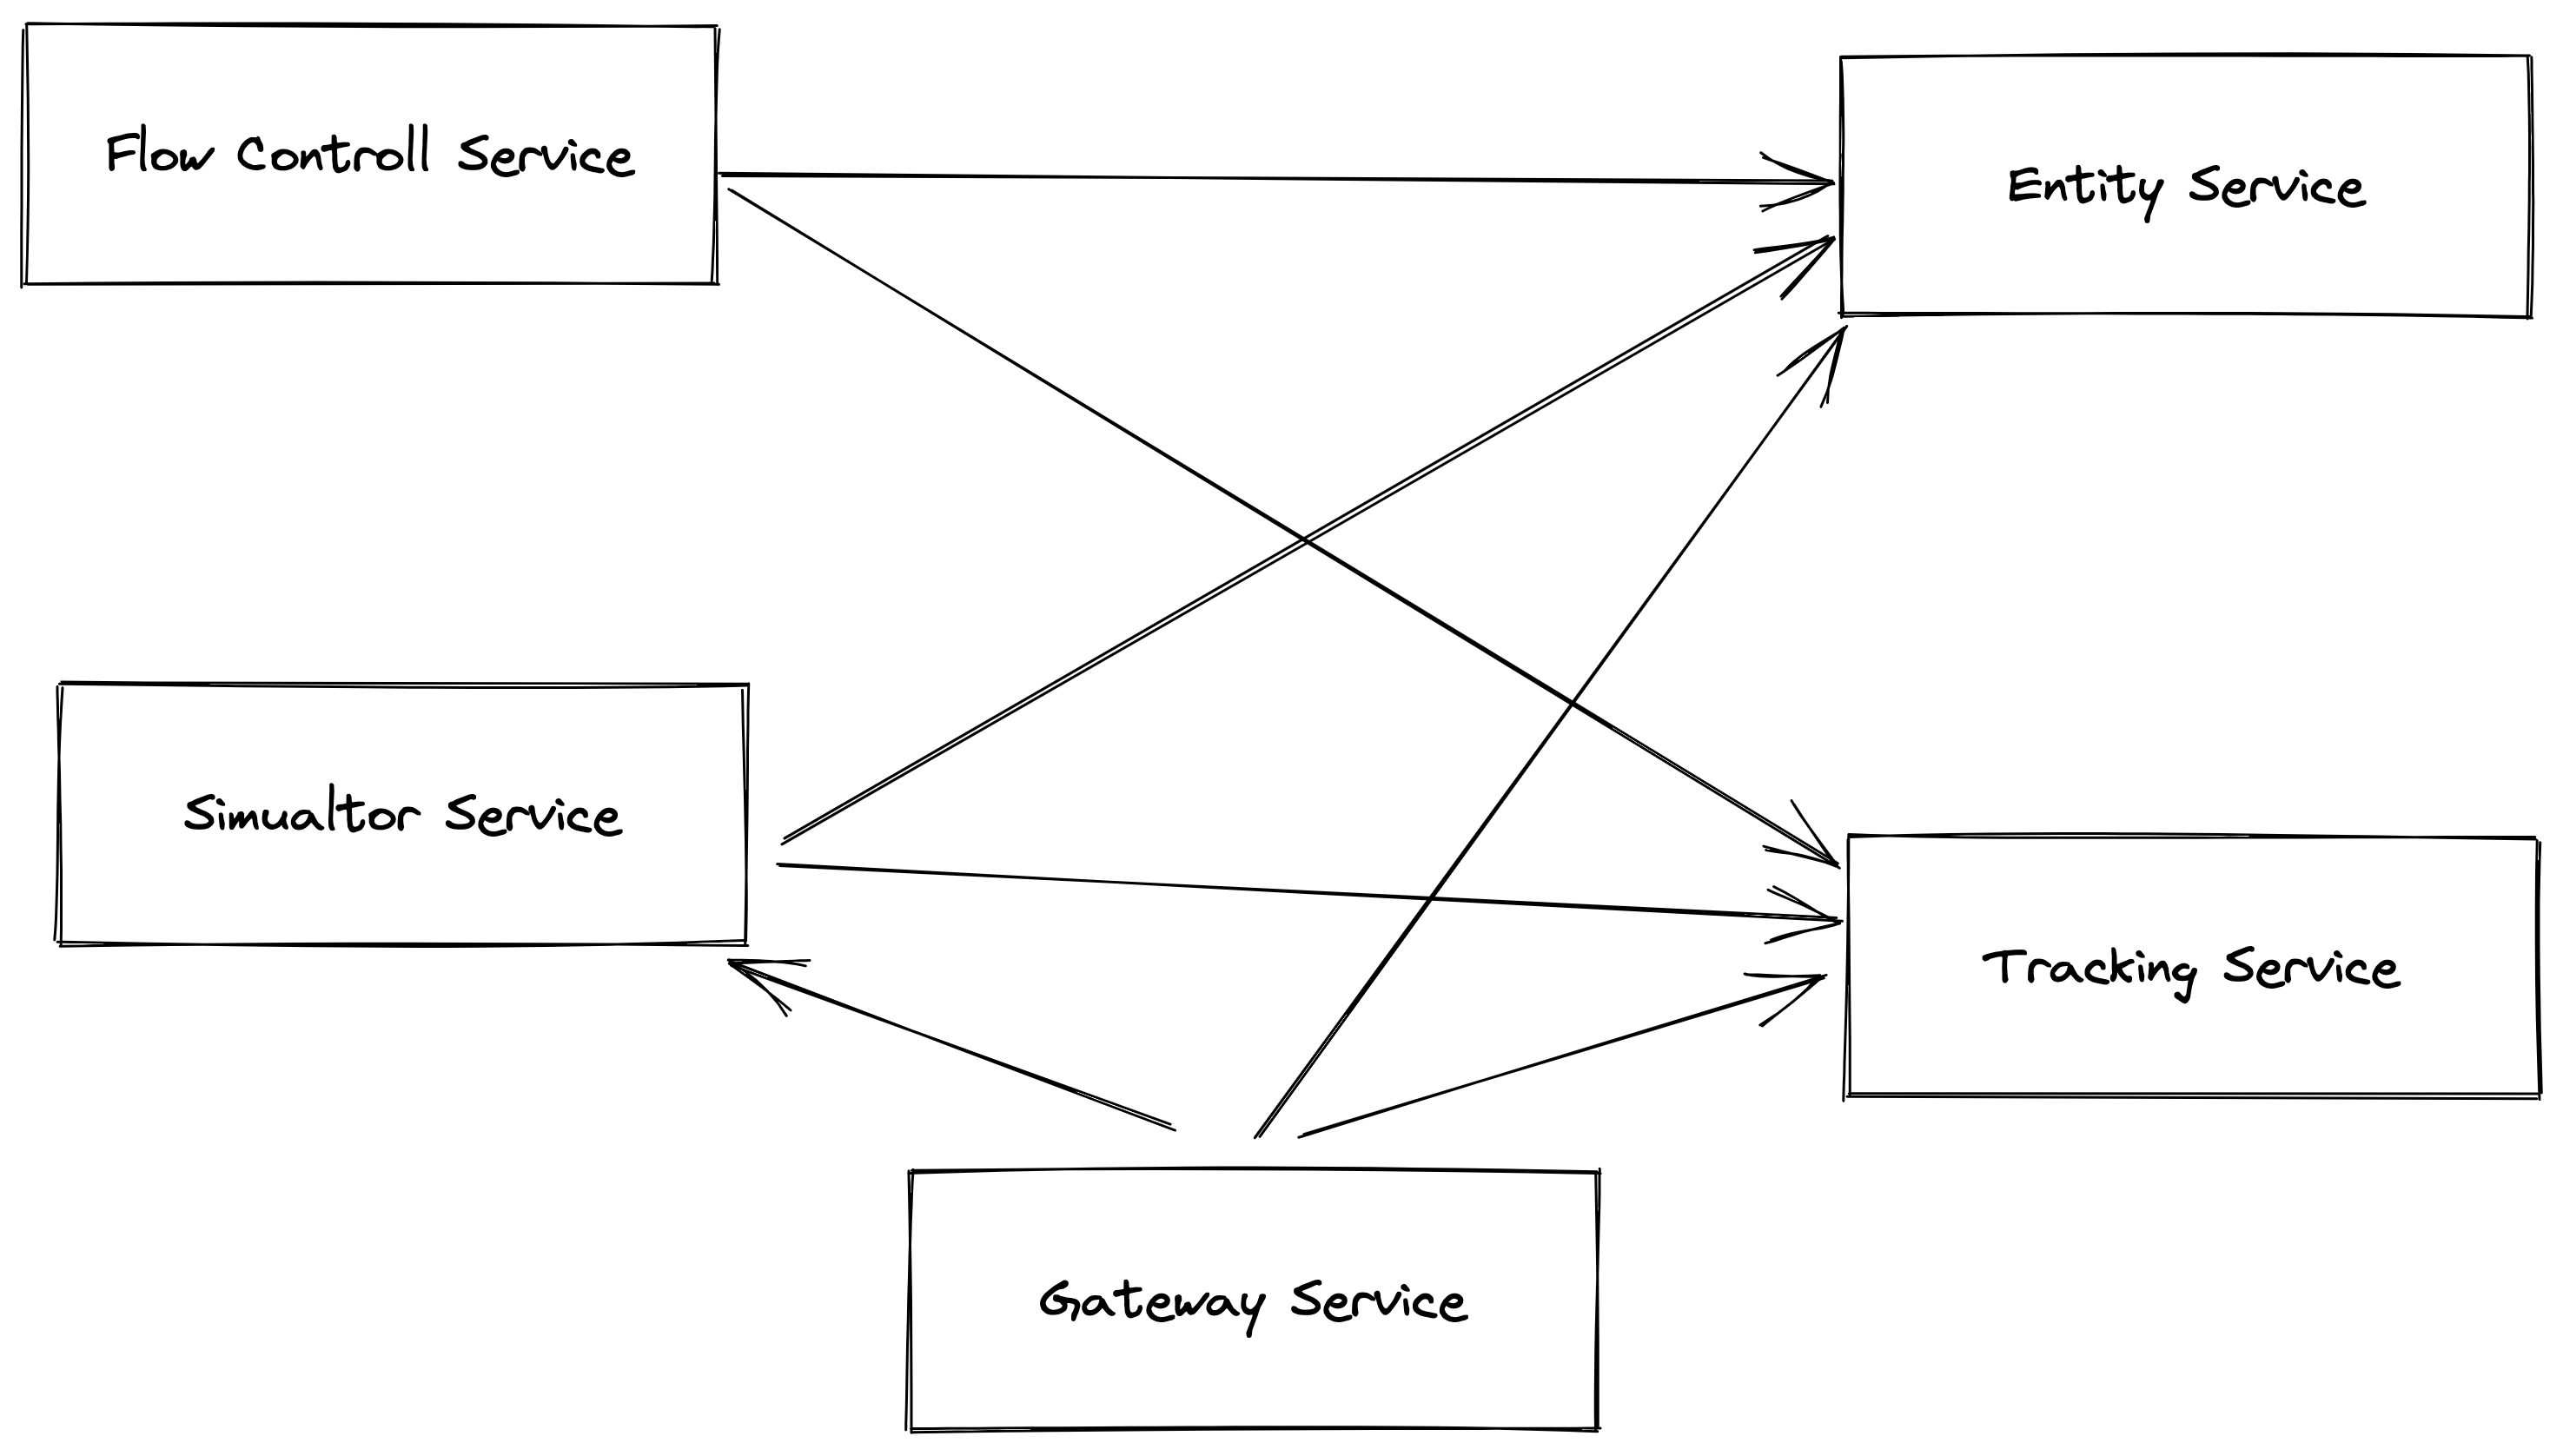
\includegraphics[width=1.02\textwidth]{./figures/rest_communication.png}
	\caption{Überblick der REST-Kommunikation}
	\label{fig:kom_rest_overview}
\end{figure}

Die Abbildung \ref{fig:kom_rest_overview} stellt die REST-Kommunikation der Services dar. 

\paragraph{Gateway}

Der Gateway kommuniziert per REST mit allen Services, welche eine solche Schnittstelle besitzen und diese auch nach außen zugänglich machen.

\paragraph{Flowcontrol-Service}

Der Flowcontrol-Service stellt keine REST-Schnittstelle bereit.
Dieser Service kommuniziert mit dem \textit{Entity-Service} sowie dem \textit{Tracking-Service}, um alle Eingaben für den Algorithmus zur Berechnung der optimalen Geschwindigkeit zu erhalten.

\paragraph{Simulator-Service}
Der Simulator-Service stellt drei REST-Endpunkte zur Verfügung.
Diese ermöglichen das Starten und Stoppen von Simulationen.
Der Simulator-Service kommuniziert mit dem \textit{Entity-Service} sowie dem \textit{Track\-ing-Service}, um einen Beenden von aktiven Simulationen zu erwirken.

\paragraph{Entity-Service}

Der Entity-Service stellt REST-Endpunkte zur Verfügung, mit welchen Metadaten und statische Informationen zu den Akteuren einer aktiven Simulation abgefragt werden können.
Der Dienst selbst sendet keine Anfragen an andere Services des Systems.

\paragraph{Tracking-Service}

Der Tracking-Service stellt REST-Endpunkte zur Verfügung, mit welchen Daten zum aktuellen Zustand der Akteure einer aktiven Simulation abgefragt werden können.
Der Dienst selbst sendet keine Anfragen an andere Services des Systems.

\subsubsection{Message Oriented Middleware}

\begin{figure}[h]
	\centering
	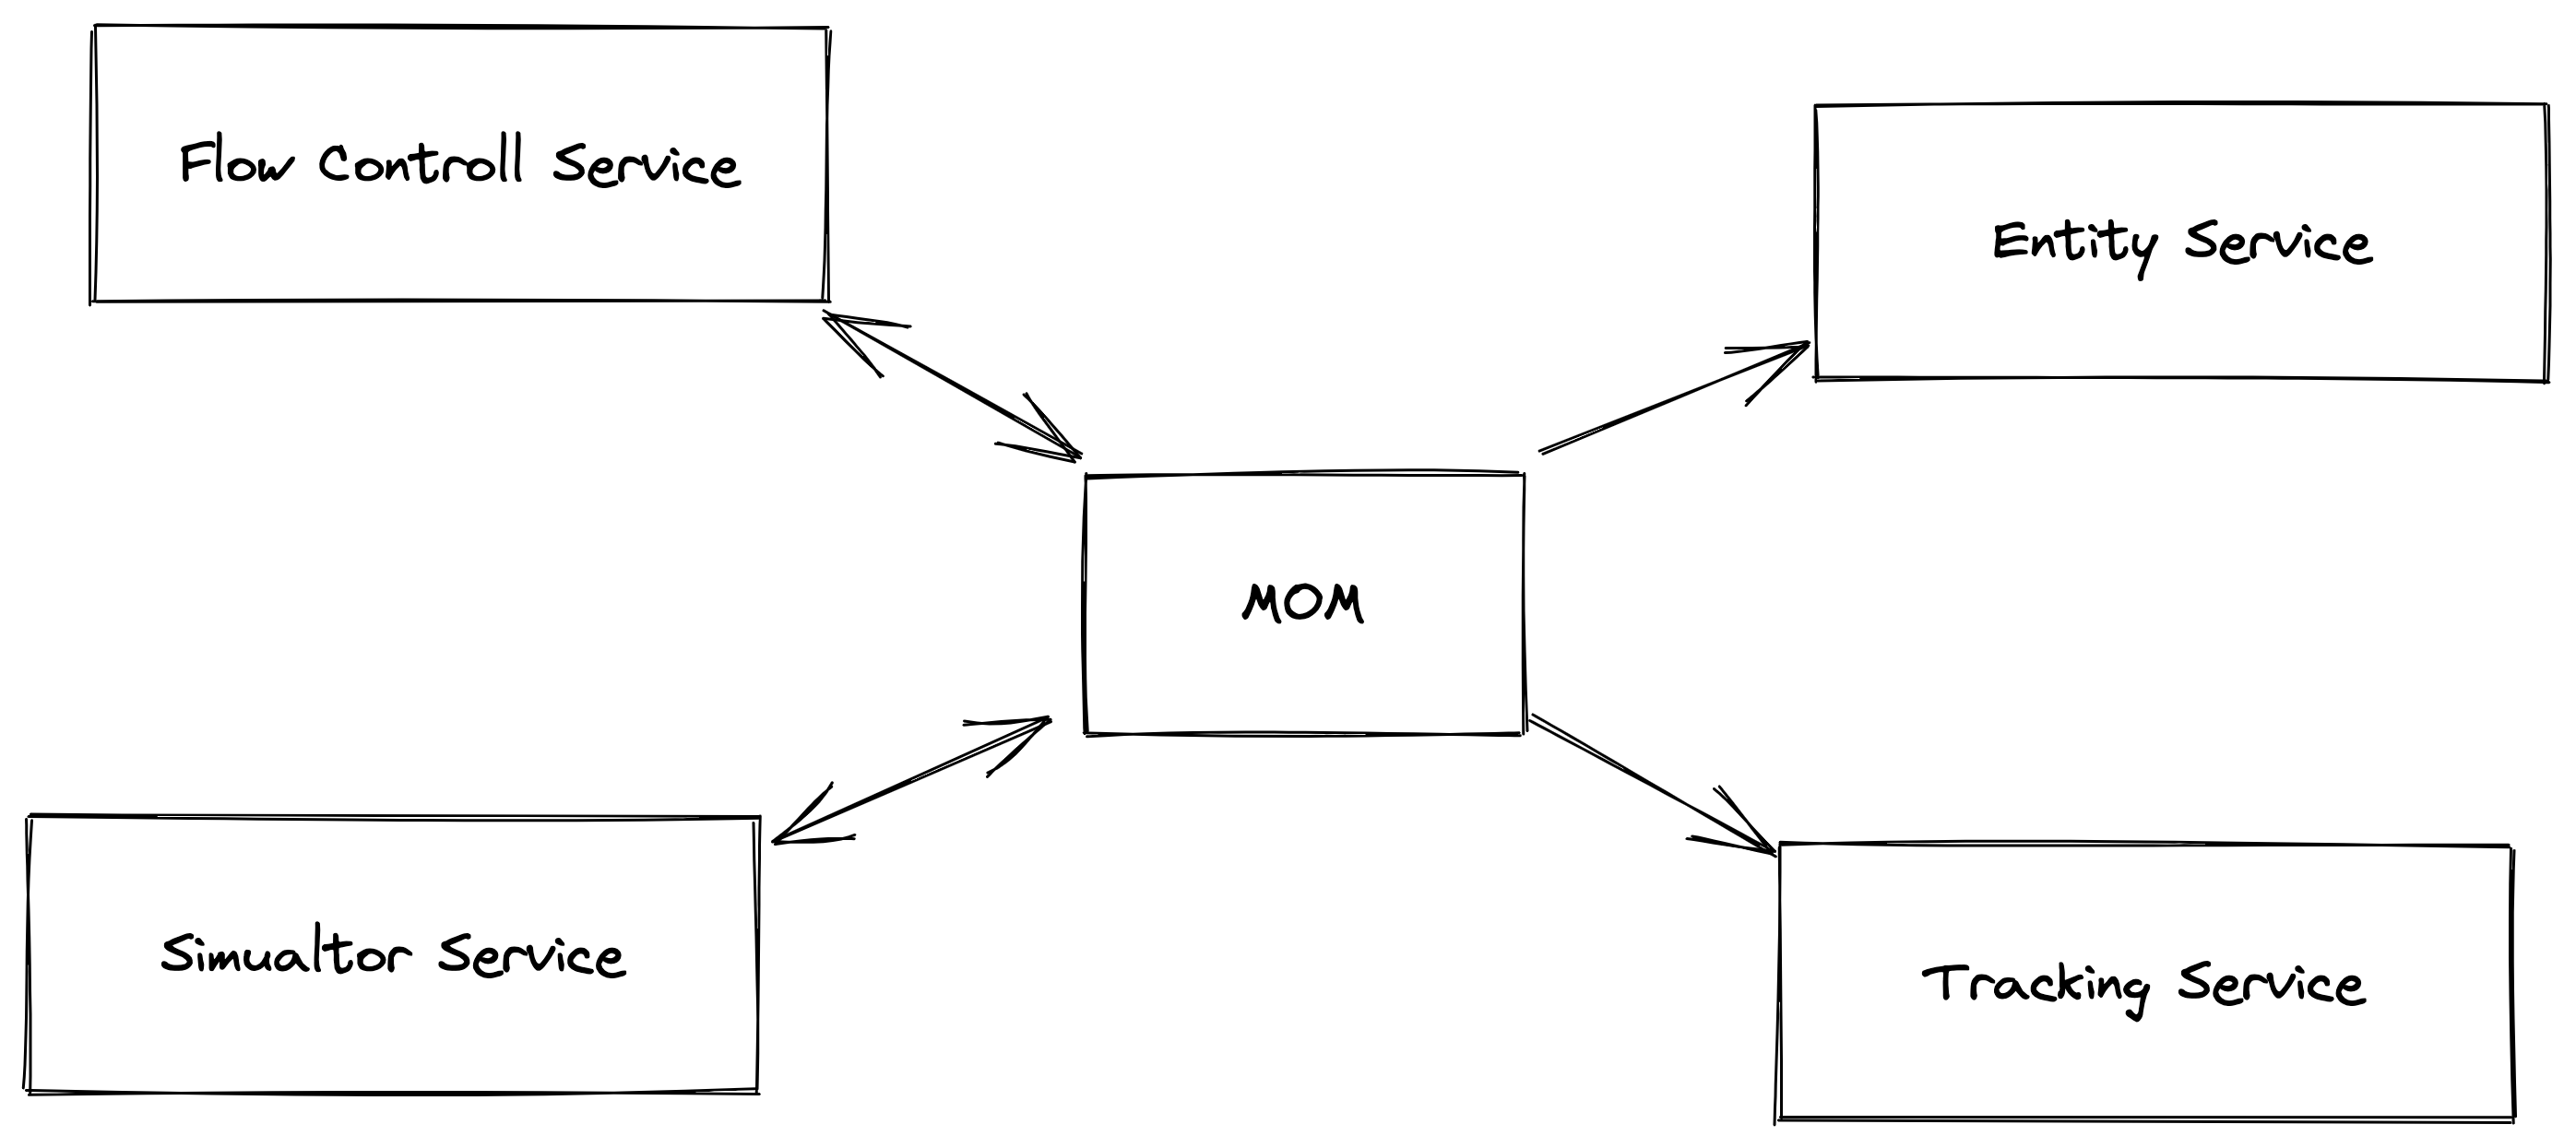
\includegraphics[width=1.02\textwidth]{./figures/mom_communication.png}
	\caption{Überblick der \enquote{MoM}- Kommunikation}
	\label{fig:kom_mom_overview}
\end{figure}

Die Abbildung \ref{fig:kom_mom_overview} bietet einen Überblick über die \enquote{MoM}-Kommunikation der Services.
Wie dort zu sehen ist, empfangen \textit{Tracking-Service} und \textit{Entity-Service} nur Daten von der \enquote{MoM} und senden selbst keine Nachrichten.
Auf der anderen Seite ist zu sehen, dass \textit{Flowcontrol-Service} und \textit{Simulator-Service} sowohl Daten an die \enquote{MoM} senden als auch empfangen. 

Insgesamt gibt es sechs Queues und einer Fanout-Exchange mit dem Namen \verb|fanout.carState|.
Die Namen der Queues sind wie folgt:
\begin{enumerate}
	\item \verb|car-state-tracking| 
	\item \verb|car-state-flow| 
	\item \verb|car| 
	\item \verb|traffic-light| 
	\item \verb|traffic-light-state| 
	\item \verb|car-speed| 
\end{enumerate}

In den folgenden Abschnitten werden die Queues sowie die Fanout-Ex\-change vorgestellt.

\begin{figure}[h]
	\centering
	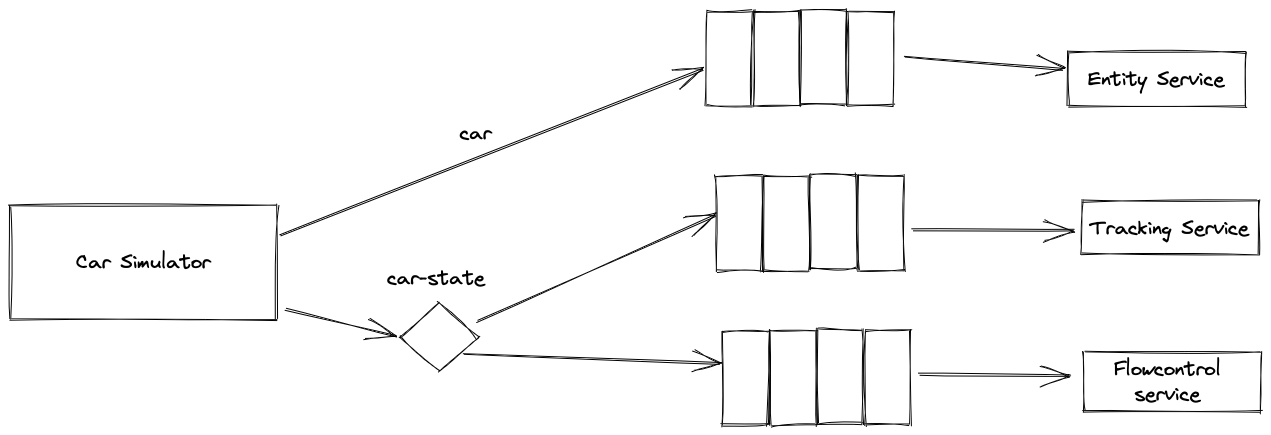
\includegraphics[width=1\textwidth]{./figures/car_simulator_mom.png}
	\caption{Verwendung der \textit{Car}, \textit{Car-State-*} und Exchange}
	\label{fig:car_simulator_mom}
\end{figure}

\paragraph{car, car-state-*, exchange}

In Abbildung \ref{fig:car_simulator_mom} ist die Verwendung der Queues \textit{Car}, \textit{Car-State-*} und der Exchange dargestellt.
Zu Beginn einer Simulation sendet der \textit{Car-Simulator} Registrierungsinformationen von Fahrzeugen an die Queue \textit{car}.
Diese Queue wird vom Entity-Service konsumiert.
Während der Simulation werden aktuelle Positionen, Geschwindigkeiten und weiteres dynamische Daten an die Fanout-Exchange gesendet (welche in der Abbildung \ref{fig:car_simulator_mom} als Raute gekennzeichnet ist).
Die Fanout-Exchange leitet diese an die beiden Queues \textit{car-state-flow} und \textit{car-state-tracking} weiter.
Diese Designentscheidung wurde getroffen, da es sich hier um ein \textit{PubSub}-Szenario und keine \textit{Competing-Consumers} handelt.

\begin{figure}[h]
	\centering
	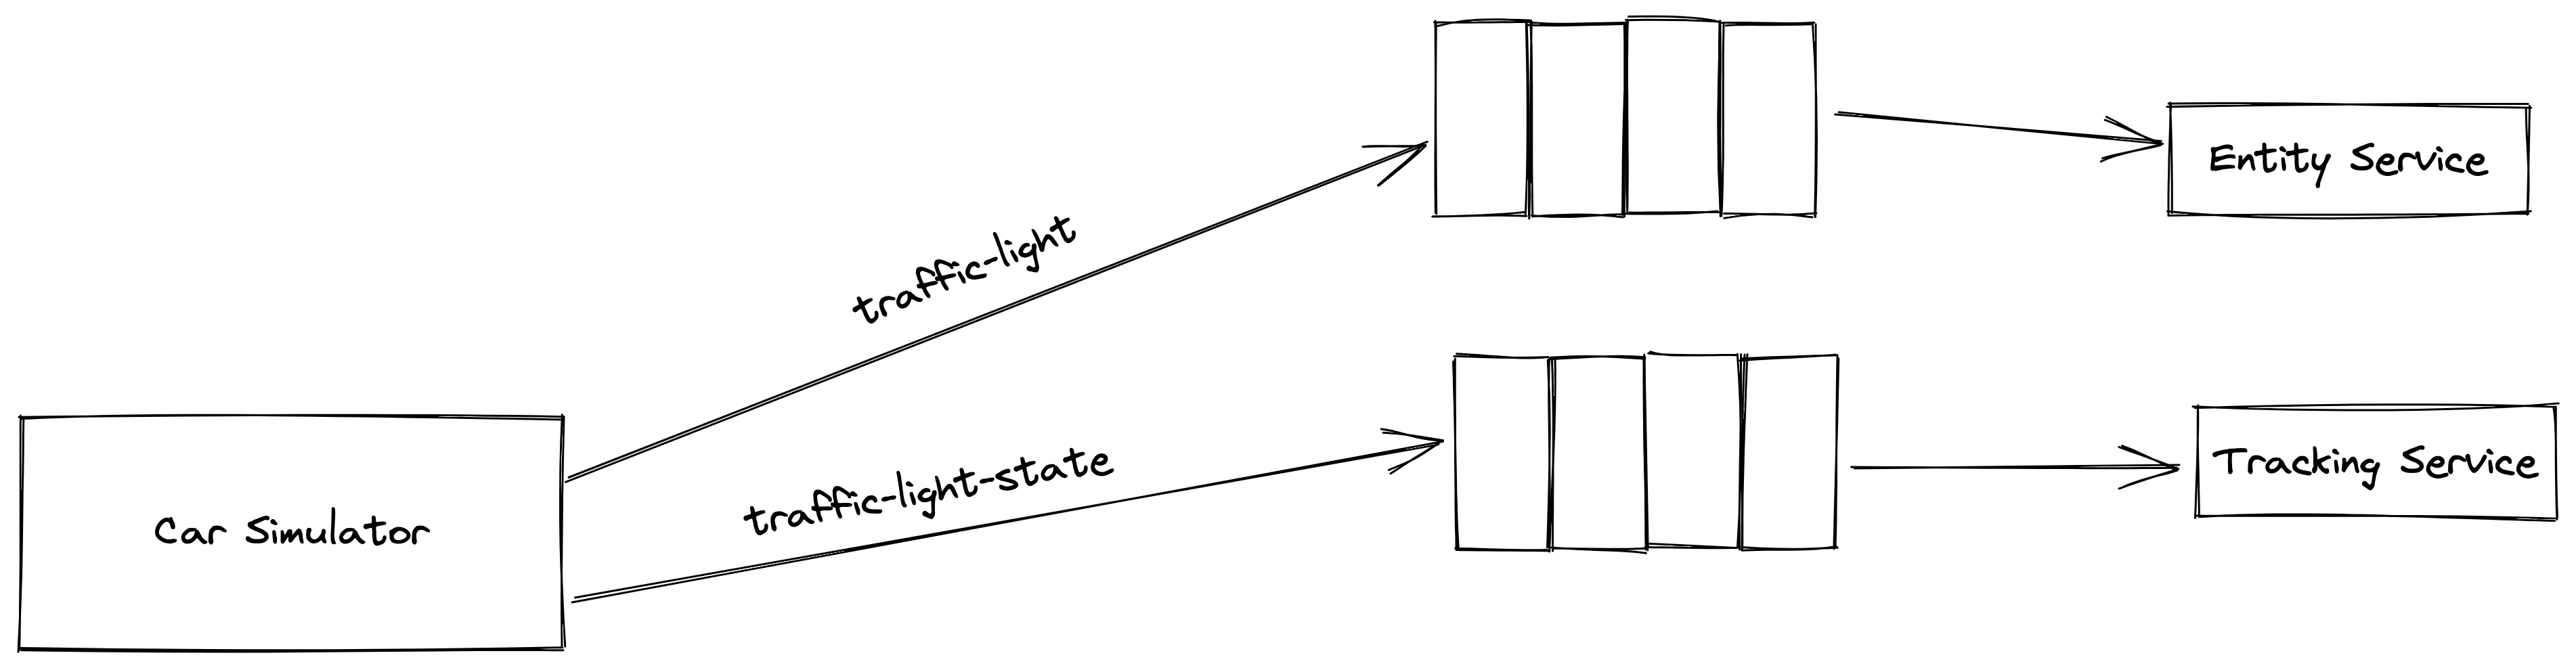
\includegraphics[width=1\textwidth]{./figures/traffic-light_simulator_mom.png}
	\caption{Verwendung der Queues \textit{traffic-light}, \textit{traffic-light-state} }
	\label{fig:light_simulator_mom}
\end{figure}

\paragraph{taffic-light, taffic-light-state-*}

In Abbildung \ref{fig:light_simulator_mom} wird die Verwendung der Queues \textit{traffic-light}, \textit{traffic-light-state} dargestellt.
Zu Beginn einer Simulation sendet der \textit{TrafficLight-Simulator} Registrierungsinformationen von Ampeln an die Queue \textit{traffic-light}.
Diese Queue wird vom Entity-Service konsumiert.
Während der Simulation werden die verbleibende Zeit einer aktiven Ampelphase sowie weitere dynamische Daten an die Queue \textit{traffic-light-state} gesendet, welche vom \textit{tracking-service} konsumiert wird.

\begin{figure}[h]
	\centering
	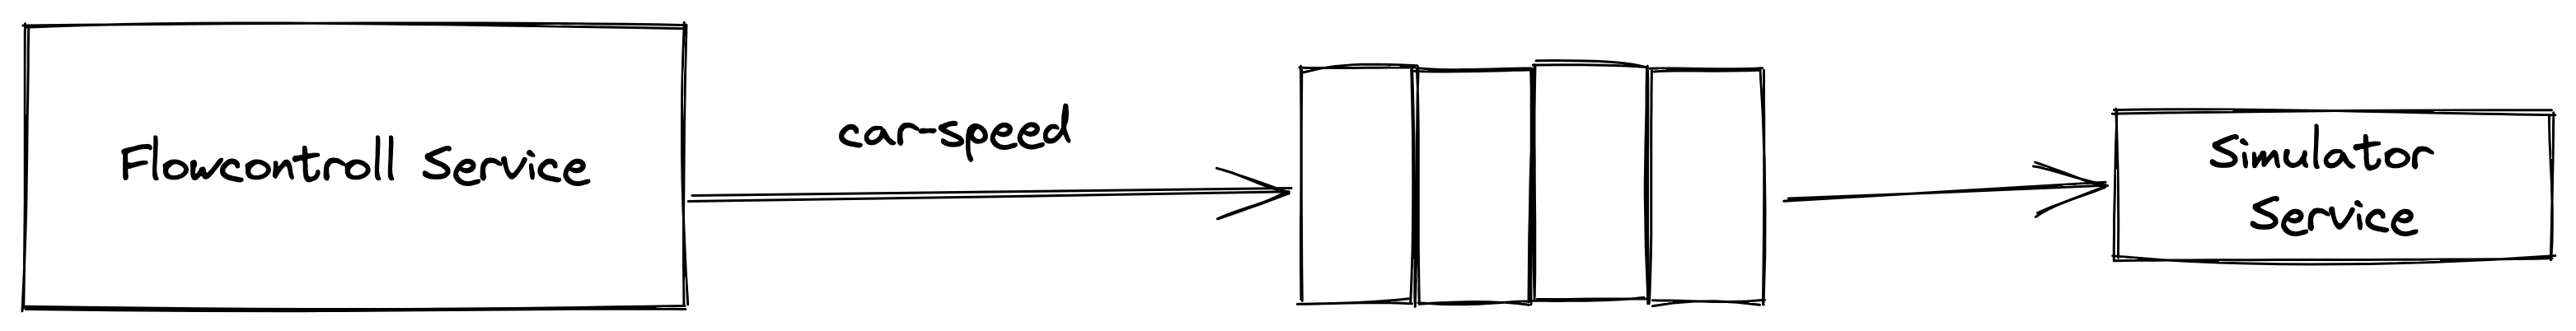
\includegraphics[width=1\textwidth]{./figures/flow_controll_speed_mom.png}
	\caption{Verwendung der Queue \textit{car-speed}}
	\label{fig:car_speed_mom}
\end{figure}

\paragraph{car-speed}

Zuletzt zeigt Abbildung \ref{fig:light_simulator_mom} die Verwendung der Queue \textit{car-speed}.
Der \textit{Flowcontrol-Service} sendet, nachdem eine optimale Geschwindigkeit für ein Fahrzeug berechnet wurde, diese mittels der Queue \textit{car-speed} and den \textit{Simulator-Service}.
